% !TeX TXS-program:compile = txs:///pdflatex/[--shell-escape]
\documentclass[10pt,landscape,a4paper]{article}
\usepackage[normalem]{ulem}
\usepackage{tikz}
\usetikzlibrary{shapes,positioning,arrows,fit,calc,graphs,graphs.standard}
\usepackage[nosf]{kpfonts}
\usepackage[t1]{sourcesanspro}
\usepackage{multicol}
\usepackage{wrapfig}
\usepackage[top=1mm,bottom=1mm,left=1mm,right=1mm]{geometry}
\usepackage[framemethod=tikz]{mdframed}
\usepackage{microtype}
\usepackage{tabularx}
\usepackage{hhline}
\usepackage{makecell}
\usepackage{mathtools}
\usepackage{listings}
\usepackage{subfig}

\DeclarePairedDelimiter{\ceil}{\lceil}{\rceil}

\newcommand\codeblue[1]{\textcolor{blue}{\code{#1}}}

\usepackage{lastpage}
\usepackage{datetime}
\yyyymmdddate
\renewcommand{\dateseparator}{-}
\let\bar\overline

\definecolor{myblue}{cmyk}{1,.72,0,.38}

\def\firstcircle{(0,0) circle (1.5cm)}
\def\secondcircle{(0:2cm) circle (1.5cm)}

\colorlet{circle edge}{myblue}
\colorlet{circle area}{myblue!5}

\tikzset{filled/.style={fill=circle area, draw=circle edge, thick},
    outline/.style={draw=circle edge, thick}}

\pgfdeclarelayer{background}
\pgfsetlayers{background,main}

\renewcommand{\baselinestretch}{.8}
\pagestyle{empty}

\let\counterwithout\relax
\let\counterwithin\relax
\usepackage{chngcntr}

\usepackage{verbatim}

\usepackage{etoolbox}
\makeatletter
\preto{\@verbatim}{\topsep=0pt \partopsep=0pt }
\makeatother

\counterwithin*{equation}{section}
\counterwithin*{equation}{subsection}
\usepackage{enumitem}
\newlist{legal}{enumerate}{10}
\setlist[legal]{label*=\arabic*.,leftmargin=2.5mm}
\setlist[itemize]{leftmargin=3mm}
\setlist[enumerate]{leftmargin=3.5mm}
\setlist{nosep}
\usepackage{minted}

\def\code#1{\texttt{#1}}

\newenvironment{descitemize} % a mixture of description and itemize
{\begin{description}[leftmargin=*,before=\let\makelabel\descitemlabel]}
    {\end{description}}

\newcommand{\descitemlabel}[1]{%
    \textbullet\ \textbf{#1}%
}
\makeatletter

\renewcommand{\section}{\@startsection{section}{1}{0mm}%
    {.2ex}%
    {.2ex}%x
    {\color{myblue}\sffamily\small\bfseries}}
\renewcommand{\subsection}{\@startsection{subsection}{1}{0mm}%
    {.2ex}%
    {.2ex}%x
    {\sffamily\bfseries}}
\renewcommand{\subsubsection}{\@startsection{subsubsection}{1}{0mm}%
    {.2ex}%
    {.2ex}%x
    {\rmfamily\bfseries}}

\def\mathcolor#1#{\@mathcolor{#1}}
\def\@mathcolor#1#2#3{%
    \protect\leavevmode
    \begingroup
    \color#1{#2}#3%
    \endgroup
}

\makeatother
\setlength{\parindent}{0pt}

\setminted{tabsize=2, breaklines}
% Remove belowskip of minted
\setlength\partopsep{-\topsep}

\setlength\columnsep{1.5pt}
\setlength\columnseprule{0.1pt}

\begin{document}
    \setlength{\abovedisplayskip}{0pt}
    \setlength{\belowdisplayskip}{0pt}

    \scriptsize
    \begin{multicols*}{4}
        \raggedcolumns
        \section{Computer Networks and the Internet}
        \subsection{What is the Internet?}
        \begin{itemize}
            \item Internet is a computer network that connects billions of computing devices.
            \item Devices connected to the internet are called \textbf{hosts} or \textbf{end systems}.
            \begin{itemize}
                \item Hosts can be further split into \textbf{clients} and \textbf{servers}.
            \end{itemize}
            \item Hosts are connected through \textbf{communication links} (e.g. fiber, copper, radio, satellite) or \textbf{packet switches} (e.g. routers and switches)
        \end{itemize}
        \subsection{Network Edge}
        \subsubsection{Access Network}
        \begin{itemize}
            \item Network that physically
            connects an end system to the first router
            \item They are what end-users connect to if they want to access the Internet
        \end{itemize}
        \subsection{Network Core}
        Network Core is the mesh of interconnected routers that links the Internet's end systems (Runs low level protocols)
        \subsubsection{Packet Switching}
        Data sent through the net in discrete chunks where each \textbf{packet} is transmitted at full link capacity (transmission rate / bandwidth)
        \begin{itemize}
            \item \textbf{Transmission rate (R)} = \# of bits transmitted into the link per second
            \item \textbf{Transmission delay} = Time needed to transmit L-bit packet into link = \textcolor{red}{$\frac{L(bits)}{R (bits/sec)}$}
            \item \textbf{Store-and-forward}: {\color{red}entire packet} must arrive at a router before it can be transmitted to the next link.
            \item \textbf{Queueing and loss:}
            \begin{itemize}
                \item packets enters a queue if {\color{red}arrival rate > transmission rate}
                \item packets can be dropped if buffer (queue) fills up
            \end{itemize}
            \item \textbf{Forwarding Tables and Routing Protocols:} Routers use these to determine the link it should forward the packet to.
            \item \textbf{Benefits:} Message segmentation \textbf{reduces delay}, \textbf{allow for retransmission} of smaller parts in case of
            corruption, and are \textbf{easier to buffer + queue} behind
            (more fair for other packets).
            \item \textbf{Drawbacks}: Packet needs to be re-arranged at destination and there is more overhead
        \end{itemize}
        \subsubsection{Circuit switching}
        Dedicated circuit per call
        \begin{itemize}
            \item end-end resources reserved for call between source \& dest
            \item call setup required
            \item circuit-like (\textbf{guaranteed}) performance
            \item circuit segment idle if not used (no sharing)
            \item commonly used in telephone networks
        \end{itemize}
        \subsubsection{Internet Structure}
        \begin{itemize}
            \item End systems access the Internet through  \textbf{access Internet Service Providers (ISPs)}
            \item Access ISPs must be interconnected so that any 2 hosts can send packet to each other
            \item Results in a network of network:
                \begin{itemize}
                    \item \textbf{Regional ISP:} ISPs that access nets in the region connect to.
                    \item \textbf{Tier-1 commercial ISP:} Provides national and international coverage. Regional ISPs connect to Tier-1 ISPs (e.g. Sprint, AT\&T)
                    \item \textbf{Internet Exchange Point (IXP):} Allows multiple Tier-1 ISPs to interconnect with each other
                    \begin{itemize}
                        \item Peering: bilateral. more expensive but much faster
                        \item IXP: multilateral, cheaper but slower
                    \end{itemize}
                    \item \textbf{Content-Provider Networks:} Private network own by company that connects their own data centres to the Internet, often bypassing tier-1 and regional ISP (e.g. Google)
                \end{itemize}
           \item If we were to connect all $N$ devices in a network, we would need $N \times{(N-1)} \slash{2}$ links\\
        \end{itemize}
        \begin{center}
            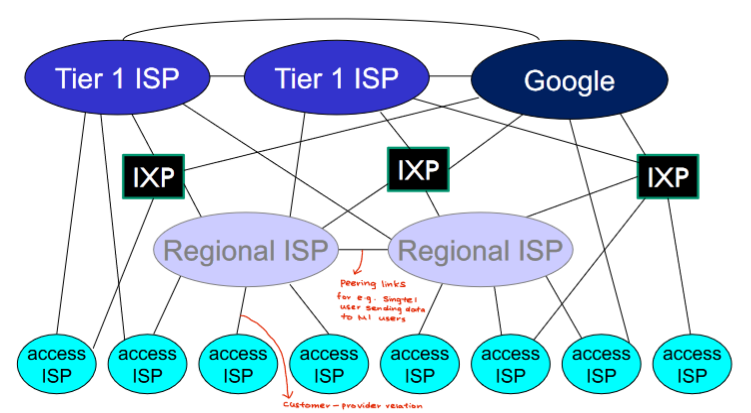
\includegraphics[scale=0.4]{internet_structure}
        \end{center}
        \subsection{Delay, Loss and Throughput in Networks}
        \subsubsection{Packet Loss}
        As the queue for router has finite capacity, a router will \textbf{drop} a packet if the queue is full and the packet will be lost. It \textbf{can be retransmitted} by previous node, source end system or not at all.
        \subsubsection{4 Sources of Packet Delay}
        \begin{itemize}
            \item \textbf{Nodal Processing (\textcolor{red}{$d_{proc}$}):} check bit errors, determine output link, typically in microseconds or less
            \item \textbf{Queueing (\textcolor{red}{$d_{queue}$}):} time waiting in output link for transmission, depends on congestion level of router. Typically in microseconds to milliseconds.
            \item \textbf{Transmission (\textcolor{red}{$d_{trans} = \frac{L}{R}$}):} L = packet length (bits), R = link bandwidth (bps), time taken to push data onto link
            \item \textbf{Propagation (\textcolor{red}{$d_{prop} = \frac{d}{s}$}):} d = length of physical link, s = propagation speed in medium ($2\times 10^8m/sec$), time taken to travel through physical link
            \item For $N-1$ routers between source host and destination host, we have: \textcolor{red}{\[d_{end-to-end}=N(=d_{proc}+d_{queue}+d_{trans}+d_{prop})\]}
        \end{itemize}
        \subsubsection{Throughput}
        \begin{itemize}
            \item Rate (bits/unit time) at which bits are transferred between sender/receiver
            \begin{itemize}
                \item \textbf{average:} rate over longer period of time (note that size of file does not matter in this case!)
                \item \textbf{instantaneous:} rate at given point in time
            \end{itemize}
        \end{itemize}
%        \subsubsection{Units}
%        \begin{itemize}
%            \item 1 byte = 8 bits
%            \item (-) Prefixes: milli, micro, nano, pico, femto, atto, zepto, yocto
%            \item (+) Prefixes: kilo, mega, giga, tera, peta, exa, zetta, yotta
%        \end{itemize}

        \subsection{Protocol Layers and Service Models}
        \textbf{Protocols}: Define format, order of messages sent and received among network entities, and actions taken on message transmission, receipt\\\\
        To provide structure to the design of network protocols,
        network designers organise protocols in layers. We are
        interested in the services that a layer offers to the \textbf{layer
        above}, i.e. the \textbf{service model} of a layer.
        \subsubsection{Why layer?}
        \begin{itemize}
            \item explicit structure \textbf{allows identification}
            \item modularization \textbf{eases maintenance}, updating of system
            \begin{itemize}
                \item change in implementation of a layer's service is transparent to the rest of the system, i.e. changing one layer \textbf{does not} affect the rest of the layers
            \end{itemize}
        \end{itemize}
        \subsubsection{5 Layers}
        \begin{itemize}
            \item \textbf{Application}: Where network applications and their application-layer protocols reside. A packet of information at this layer is called a \textbf{message}. Examples: FTP, SMTP, HTTP
            \item \textbf{Transport}: Transports application-layer messages between application endpoints. A transport-layer packet is called a \textbf{segment}. Examples: TCP, UDP
            \item \textbf{Network}: routing of \textbf{datagrams} from source to destination. Examples: IP, routing protocols
            \item \textbf{Link}: Data transfer of \textbf{frames} between neighbouring network elements (nodes). Examples: Ethernet, 802.11 (WiFi), PPP
            \item \textbf{Physical}: bits ``on the wire''. Link dependent and transmission medium-dependent
        \end{itemize}

        \section{Application Layer}
        \textbf{Goal}: Write programs that run on different end systems, communicate over the network (e.g. web server software $\leftrightarrow$ browser software)\\
        Note that network-core devices (routers) have \textbf{no application or even transport layer} which allows for rapid application development.
        \subsection{Principles of Network Applications}
        \subsubsection{Client-Server Architecture}
        \begin{itemize}
            \item \textbf{Server}: always-on, waits for incoming requests, provides requested service to client, data centres for scaling, has \textbf{permanent IP address}
            \item \textbf{Client}: initiates contact with server, typically requests service from server, may have \textbf{dynamic IP addresses}, do not communicate with each other, may be intermittently connected
        \end{itemize}
        \subsubsection{Peer-to-Peer (P2P)}
        \begin{itemize}
            \item No always-on server
            \item Arbitrary \textbf{end systems directly communicate}
            \item Peers request and provide services to other peers
            \item \textbf{Self-scalability}: new peers bring new service capacity, as well as new service demands
            \item Peers are intermittently connected and change IP addresses (lead to complex management)
%            \item e.g. BitTorrent, Limewire, Kazaa
        \end{itemize}
        \subsection{Process Communication}
        \subsubsection{Sockets}
        \begin{itemize}
            \item A \textbf{software interface} (between application \& transport layer) that a process uses to send messages into, and receive messages from the
            network. Uses \textbf{IP address and a port number} as identifier.
            \item \textbf{IP Address:} 32-bit Integer that uniquely identifies a host
            \item \textbf{Port Number:} 16-bit integer that identify what services a process is using (e.g. HTTP Server: 80, mail server: 25, DNS: 53)
        \end{itemize}
        \subsubsection{Transport Services}
        \begin{itemize}
            \item \textbf{Data integrity}: 100\% reliable (e.g. file transfers, web transactions) vs tolerant to data loss (e.g. audio, video stream, multimedia)
            \item \textbf{Timing}: some apps require low delay (latency) to be ``effective'' (e.g. interactive games, zoom)
            \item \textbf{Throughput:} require minimum amount of throughput to be ``effective'' (e.g. gaming)
            \item \textbf{Security:} encryption scheme, data integrity\\
        \end{itemize}
        \begin{center}
            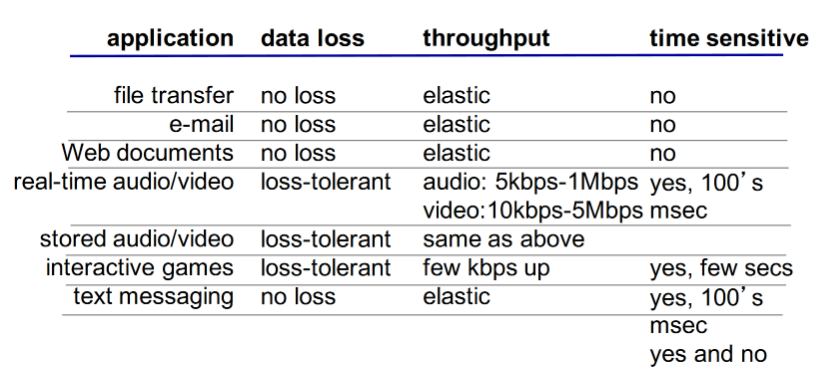
\includegraphics[width=0.7\columnwidth]{service_req}
        \end{center}
        \subsubsection{Transport-Layer Protocols}
        \begin{tabularx}{\columnwidth}{|X|X|}
            \hline
            \textbf{TCP} & \textbf{UDP} \\
            \hline
            \textbf{Reliable} data transfer & \textbf{Unreliable} data transfer\\
            \hline
            \textbf{Flow control}: sender won't overwhelm receiver & \textbf{No flow control}\\
            \hline
            \textbf{Congestion control}: throttle sender when network is overloaded & \textbf{No congestion control}\\
            \hline
            \textbf{Connection-oriented:} setup required between client and server & \textbf{No setup} needed\\
            \hline
            \textbf{Does not provide}: timing, minimum throughput guarantee, security & \textbf{Does not provide}: timing, throughput guarantee, security \\
            \hline
        \end{tabularx}
        \begin{itemize}
            \item Why UDP?
            \begin{itemize}
                \item UDP has less overhead and complexity and has its uses in multimedia where data integrity is not as important and delay might be shorter
            \end{itemize}
        \end{itemize}
        \begin{center}
            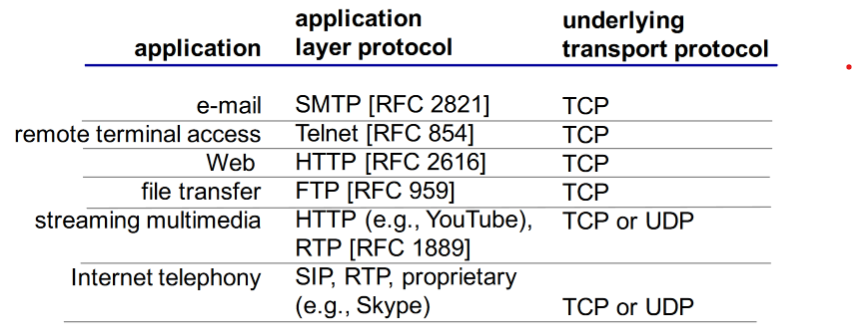
\includegraphics[width=0.8\columnwidth]{app_transport}
        \end{center}
        \subsubsection{Definition of App-layer Protocols}
            \begin{itemize}
                \item \textbf{Types of Messages exchanged,} e.g. request, response
                \item \textbf{Message syntax}, e.g. message fields and how they are delineated
                \item \textbf{Message semantics}: meaning of information in fields
                \item \textbf{Rules} for when and how application send and respond to messages\\
            \end{itemize}

            There are also open protocols defined in RFCs (Request for Comments) such as HTTP (allows for interoperability) and some proprietary protocols (e.g. Skype)
        \subsection{Web and HTTP}
        \subsubsection{Web Page}
        \begin{itemize}
            \item consists of a base HTML file and several referenced objects
            \item objects can be HTML file, JPEG image, Java applet, audio file etc.
            \item object is addressable by a URL:
                \begin{itemize}
                    \item \textbf{Hostname}: www.comp.nus.edu.sg
                    \item \textbf{Path name}: /
                    \textasciitilde cs2105/img/lect1.pdf
                \end{itemize}
        \end{itemize}
        %\vfill\null
        %\columnbreak
        \subsubsection{HTTP}
        \begin{itemize}
            \item \textbf{HyperText Transfer Protocol} is the Web's \textbf{application layer} protocol
            \item \textbf{Client/server model}: Client is the browser that requets, receives and ``displays'' web objects whereas the server is a Web Server that sends objects in response to requests
            \item \textbf{Over TCP} (Reliable!)
            \item \textbf{Stateless}: server maintains no information about past client requests
        \end{itemize}
        \subsubsection{Persistent HTTP}
        \begin{itemize}
            \item \textbf{Multiple objects} can be sent \textbf{over single TCP} connection
            \item TCP connection is left open after sending response
            \item \textbf{Persistent with pipelining}: client may send requests as soon as it encounters a referenced object -- as little as 1RTT for \textcolor{red}{all} referenced objects.
        \end{itemize}
        \subsubsection{Non-Persistent HTTP}
        \begin{itemize}
            \item At most 1 object sent over a TCP connection (TCP connection is closed after each request)
            \item downloading {\color{red}multiple objects requires multiple connections}
            \item Requires 2 RTTs per object (1 to initiate TCP connection, 1 to request the file), and 2 RTTs get the initial HTML file
            \item Response time $= (2\times RTT + $ file transmission time) / object
            \item incurs \textbf{overhead} for each TCP connection $\rightarrow$ solution is to \textbf{open parallel TCP connections}
        \end{itemize}
        * \textbf{RTT}: time for a small packet to travel from client to server and back (does not include transmission delay!)
        \[RTT = d_{proc}+d_{queue}+d_{prop}\]
        \subsubsection{HTTP Request Format}
        * Note that it is \textbf{not possible to find IP address} of Host in the HTTP header
        \begin{center}
            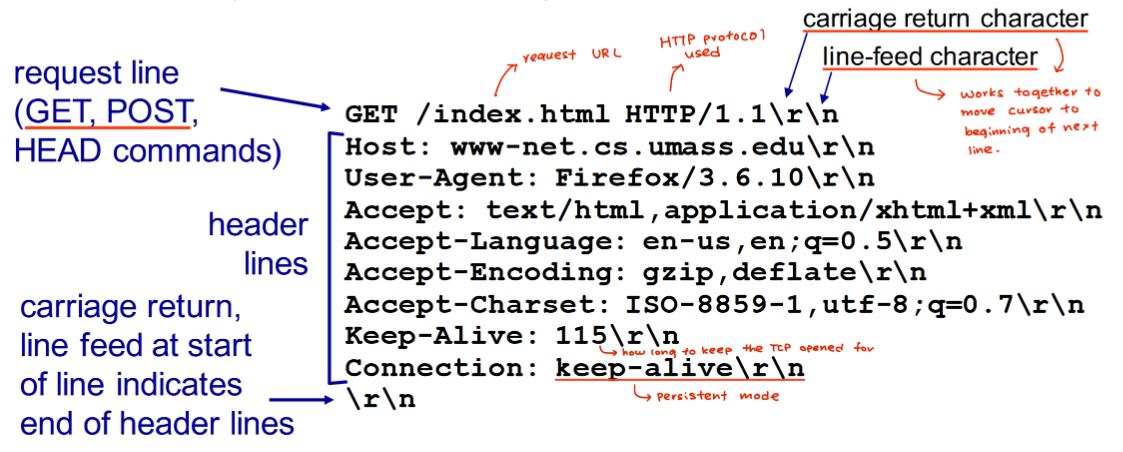
\includegraphics[width=0.8\columnwidth]{http_msg}
            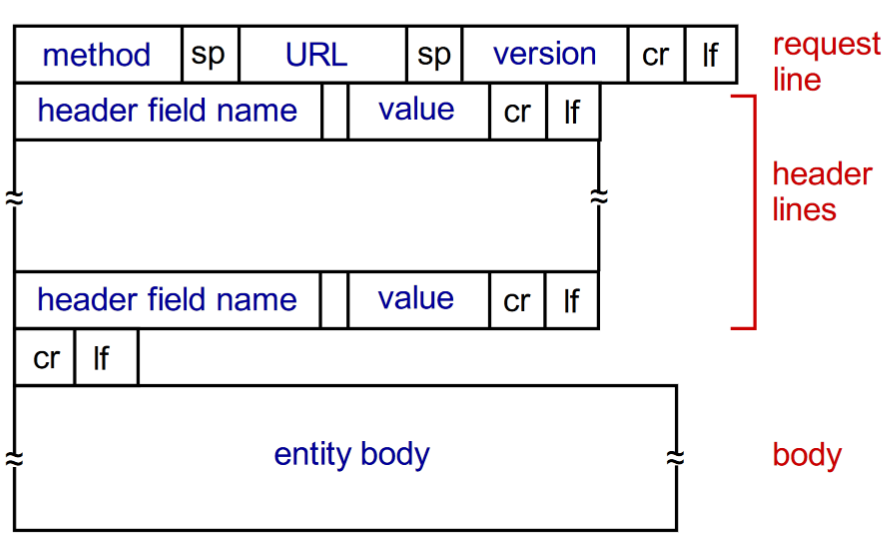
\includegraphics[width=0.6\columnwidth]{http_general}
        \end{center}
        \subsubsection{HTTP Method Types}
        \begin{itemize}
            \item \textbf{HTTP/1.0} (Default to Non-Persistent):
            \begin{itemize}
                \item \texttt{GET}: Gets an object
                \item \texttt{POST}: Requests web server to put data in body of message, typically used for sending form data
                \item \texttt{HEAD}: asks server to leave requested object out of response (mostly for debugging)
            \end{itemize}
            \item \textbf{HTTP/1.1} (Default to Persistent):
            \begin{itemize}
                \item \texttt{GET, POST, HEAD}
                \item \texttt{PUT}: uploads file in entity body to path specified in URL
                \item \texttt{DELETE}: deletes file specified in URL
            \end{itemize}
        \end{itemize}
        \subsubsection{HTTP Response Status Codes}
        \begin{itemize}
            \item \texttt{\textbf{200 OK}}: Request succeeded, requested object later in this msg
            \item \texttt{\textbf{301 Moved Permanently}}: requested object moved, new location specified later in this msg (Location:)
            \item \texttt{\textbf{400 Bad Request}}: request msg not understood by server
            \item \texttt{\textbf{404 Not Found}}: requested document not found on this server
            \item \texttt{\textbf{500 HTTP Version Not Supported}}
        \end{itemize}
        \subsection{Cookies}
        As HTTP is stateless, we need cookies to help carry states. Cookies has four components:
        \begin{enumerate}
            \item cookie header line of HTTP response message
            \item cookie header line in next HTTP request message
            \item cookie file is stored on user's host and is managed by user's browser
            \item back-end database at website\\
        \end{enumerate}
        Cookies are typically used for: authorization, shopping carts, recommendations, user session state (Web email). The state is maintained at sender/receiver over \textbf{multiple transactions}
        \vfill\null
        \columnbreak
        \subsubsection{Conditional GET}
        Web heavily \textbf{utilises caching to reduce response time} by caching objects in a proxy server (typically much closer to clients). If a request object is in the proxy server, cache returns the object else it will request object from origin server. (lowers link utilisation)\\\\
        Since there is a cache, we must handle and prevent transferring stale objects. This is done through a \texttt{\textbf{If-Modified-Since: <data>}} header line which returns a \texttt{\textbf{200 OK}} and returns new object if data has been modified, else \texttt{\textbf{304 Not Modified}} and no object if data is not modified.
        \subsection{DNS: The Internet's Directory Service}
        The \textbf{Domain Name System} helps to map hostnames (e.g. google.com) to their IP address and vice versa so we as humans do not have to remember individual IP addresses for websites. (Default port 53)
        \begin{itemize}
            \item \textbf{Distributed, Hierarchical Database} in the Application Layer
            \item \textbf{Root Server}: answers requests for records in the root zone by returning a list of the authoritative name servers for the appropriate TLD
            \item \textbf{DNS Caching}:
            \begin{itemize}
                \item cache entries timeout after some time (\textbf{TTL} - Time to live)
                \item TLD servers are typically cached in local name servers $\rightarrow$ root name servers are often not visited
                \item cached-entries \textbf{may be out of date} $\rightarrow$ if a host changes IP address, it may not be known until TTL expires
            \end{itemize}
            \item Runs over \textbf{UDP}
        \end{itemize}
        \subsubsection{Local DNS name server}
        \begin{itemize}
            \item when host makes DNS query, first sent to the Local DNS server
            \item contains local cache of recent name-to-address translation pairs (but \textbf{might be out of date})
            \item acts as proxy to forward query into hierarchy
            \item \textbf{does not strictly belong to hierarchy}
        \end{itemize}
        \subsubsection{Root name server}
        \begin{itemize}
            \item contacted by local name server that cannot resolve name
            \item provides IP address of TLD (Top Level Domain e.g. .com, .gov, .sg) servers
        \end{itemize}
        \subsubsection{Authoritative servers}
        \begin{itemize}
            \item organization's owned DNS servers that provides authoritative hostname to IP mappings for organization's named hosts
            \item maintained either by organization or service providers
        \end{itemize}
%        \subsubsection{Resource Records (RR)}
%        Stores mapping between hostnames and IP addresses, 4-tuple \texttt{(name, value, type, ttl)}
%        \begin{itemize}
%            \item type = A, \texttt{name} is hostname, \texttt{value} is IP address
%            \item type = NS, \texttt{name} is domain, \texttt{value} is hostname of authoritative name server for the domain
%            \item type = CNAME, \texttt{name} is alias for some canonical name, \texttt{value} is the canonical name
%            \item type = MX, \texttt{value} is the name of mail server assoc with \texttt{name}
%        \end{itemize}
        \subsubsection{DNS Name Resolution}
        \begin{itemize}
            \item \textbf{Iterative query}: Local DNS server makes DNS requests one by one in the hierarchy
            \item \textbf{Recursive query} (rarely used): each server in the hierarchy asks one server higher in the hierarchy (heavy load on root DNS server)
        \end{itemize}
        \begin{minipage}{\columnwidth}
            \makeatletter
            \newcommand{\@captype}{figure}
            \makeatother
            \centering
            \subfloat[Recursive]{%
                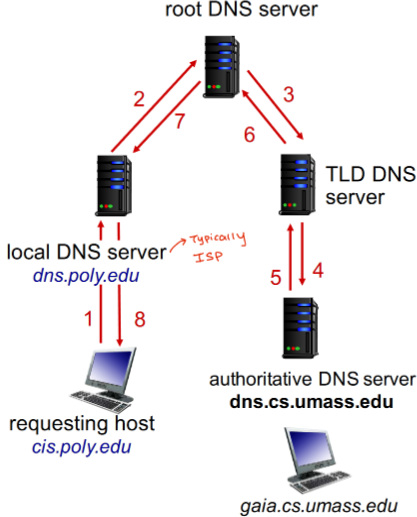
\includegraphics[width=0.4\textwidth]{recursive_dns}%
            }\qquad%
            \subfloat[Iterative]{%
                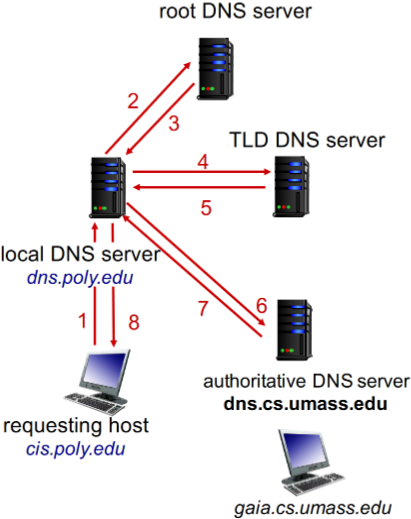
\includegraphics[width=0.4\textwidth]{iterative_dns}%
                %
            }
        \end{minipage}

        \section{Socket Programming}
        \textbf{Socket}: the software interface between app processes and transport layer. Allows for communication between processes over the Internet.\\\\
        Relies on:
        \begin{enumerate}
            \item \textbf{Port Number}: 16-bit unsigned integer (0-1023 are reserved)
            \item \textbf{IP Address}: 32-bit unsigned integer
        \end{enumerate}
        \subsection{UDP (User Datagram Protocol)}
        \begin{itemize}
            \item \textbf{unreliable} datagram, \textbf{connectionless}
            \item \textcolor{red}{no handshaking} before sending data
            \item sender (client) explicitly attaches destination IP address and port number to {\color{red}each packet}
            \item receiver (server) extracts sender IP address and port number from the received packet
            \item transmitted data \textbf{may be lost} or \textbf{received out-of-order}
        \end{itemize}
        * For clients, port number can be random whereas server port number must be assigned
        \subsection{TCP (Transmission Control Protocol)}
        \begin{itemize}
            \item reliable \textbf{byte stream}, connection-oriented
            \item When client creates socket, client TCP establishes a connection to server TCP. (Server must have ``welcome socket'')
            \item When contacted by client, server TCP creates a {\color{red}new socket} (with same port number) for server process to communicate with that client
            \item Allows server to talk with multiple clients individually.
            \item Communicates as if there is a pipe between 2 processes, sending process doesn't need to attach a destination IP address and port number in each sending attempt.
        \end{itemize}
        \begin{tabularx}{\columnwidth}{|X|X|}
            \hline
            \textbf{UDP} & \textbf{TCP} \\
            \hline
            Server uses {\color{red}one socket} to serve all clients {\tiny (n clients -> 1 socket)} & Server creates a {\color{red}new socket} for each client {\tiny (n clients -> n+1 sockets)}\\
            \hline
            No connection is established before sending data & Client establishes connection to server\\
            \hline
            Sender explicitly attaches {\color{red}destination IP address $+$ port\#} & Server uses {\color{red}connection} to identify client\\
            \hline
            Unreliable datagram: Data may be lost, received out-of-order & Reliable stream pipe: data guaranteed to be received in order\\
            \hline
        \end{tabularx}
        \section{UDP, Reliable Data Transfer}
        \subsection{Transport-layer Services and Protocols}
        \begin{itemize}
            \item provides \textbf{logical communication} (allows processes to feel like they are directly connected to each other) between app processes running on different hosts
            \item \textbf{Sender}: Breaks app messages into {\color{red}segments}, passes them to network layer
            \item \textbf{Receiver}: Reassembles segments into message, passes it to app layer
            \item Primarily uses 2 protocols:
            \begin{enumerate}
                \item TCP (reliable, more overhead, slower)
                \item UDP (unreliable, less overhead, faster)
            \end{enumerate}
        \end{itemize}
        \subsection{Transport vs Network layer}
        \begin{itemize}
            \item Transport layer: logical communication between \textcolor{red}{processes}
            \begin{itemize}
                \item relies on and enhances network layer services
            \end{itemize}
            \item network layer: logical communications between \textcolor{red}{hosts}/interfaces
            \begin{itemize}
                \item unreliable ``best-effort'' (relies on TCP for reliability)
            \end{itemize}
        \end{itemize}
        \subsection{Connectionless Transport: UDP}
        \begin{itemize}
            \item UDP adds very little on top of IP
            \begin{itemize}
                \item \textbf{Multiplexing} at sender (aggregate packets that needs to be transported out)
                \item \textbf{Demultiplexing} at receiver (determines which packets are for which processes)
                \item \textbf{Checksum}
            \end{itemize}
            \item UDP transmission is unreliable, often used by streaming multimedia app (loss tolerant \& rate sensitive apps)
        \end{itemize}
        \subsubsection{Why UDP?}
        No connection establishment (less delay), simple (no connection state at sender, receiver), small header size, no congestion control (UDP can send data without worrying about data loss)
        \subsubsection{Connectionless De-multiplexing}
        When UDP receiver receives a UDP segment:
        \begin{itemize}
            \item Check destination port number in segment, and direct that segment to the socket with that port number.
            \item basically same dest. port \# $\rightarrow$ same socket at destination
        \end{itemize}
        \subsubsection{UDP Header}
        \begin{center}
            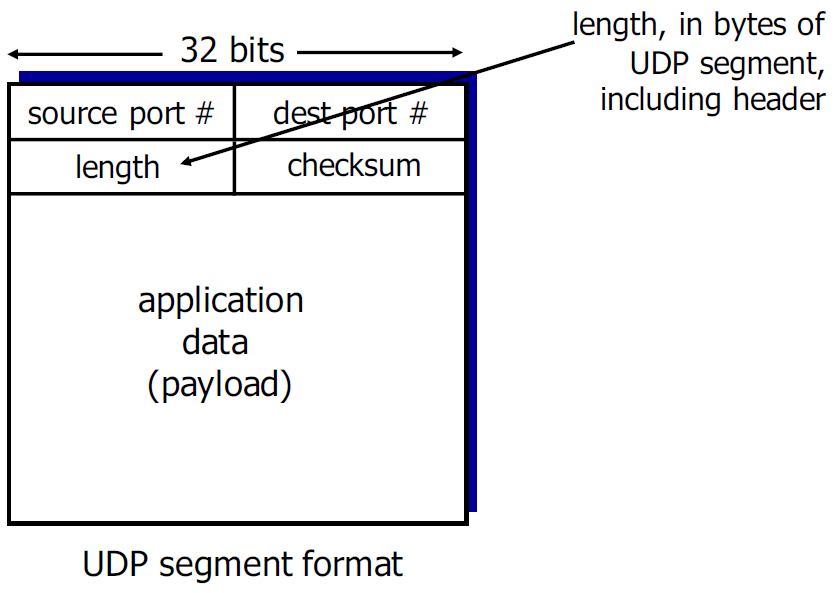
\includegraphics[width=0.4\columnwidth]{udp_header}
        \end{center}
        * Note that the minimum length of UDP segment is 8 bytes which is just the header itself
        \subsubsection{UDP Checksum}
        \begin{enumerate}
            \item Treat UDP segment as sequence of 16-bit integers
            \item Apply binary addition
            \item Add carry to result (if any)
            \item Compute 1's complement to get the UDP checksum
        \end{enumerate}
        Result of adding checksum and the original sum should give all 1's. Also note that UDP checksum is done in complement with other checksums (in network layer) to ensure reliable data transfer (passing UDP checksum alone is not guaranteed that no bit error occurred)
        \subsection{Principles of Reliable Data Transport}
        To build a reliable transport layer protocol, we have to handle:
        \begin{descitemize}
            \item Packet corruption
            \item Packet loss
            \item Packet reordering
            \item Packet delay (arbitrarily long)
        \end{descitemize}
        \subsubsection{RDT 1.0}
        \textbf{Assumption}: Underlying channel is perfectly reliable (no bit errors and no loss of packets).
        \begin{enumerate}
            \item (Sender) Make packet and send packet to receiver using network layer.
            \item (Receiver) Extract packet from network layer and deliver data to application.
        \end{enumerate}
        \subsubsection{RDT2.0}
        \textbf{Assumption}: Underlying channel may flip bits i.e. corruption. We use the stop and wait protocol (server send one packet at a time then wait for recv response).
        \begin{enumerate}
            \item (Sender) Make packet and send packet to receiver.
            \item (Receiver) Check if packet is corrupt. If not corrupt, deliver data to application and send ACK to sender, else just send NAK to sender.
            \item (Sender) If received NAK, resend the same packet, else go to step 1 for next packet.
        \end{enumerate}
        \textbf{Problems}: If ACK or NACK are corrupted, there is no guaranteed way to recover. If we simply resend the packet, the receiver will not know it’s a duplicate.
        \subsubsection{RDT2.1}
        \textbf{Assumption}: Same as rdt 2.0 - corruption. In addition to what is covered in rdt 2.0, we now add a sequence number to the packet. This number alternates between 1 and 0. Duplicates are detected using sequence number.
        \begin{enumerate}
            \item (Sender) Sends pkt0.
            \item (Receiver) Sends ACK or NAK.
            \item (Sender) If NAK or corrupted message received, retransmit message. Else send pkt1.
            \item (Receiver) If duplicate pkt0 is received, drop it and reply ACK. Else continue as per usual.
        \end{enumerate}
        \subsubsection{RDT2.2}
        \textbf{Assumption}: Same as rdt 2.0 and 2.1 - corruption. In addition to what is covered in rdt 2.1, we now explicitly include the sequence number of the packet being acknowledged, removing the need for a NAK. From the sender’s perspective, we basically resend current packet if a duplicate ACK is received.
        \begin{enumerate}
            \item (Sender) Sends pkt0.
            \item (Receiver) Sends ack1 if corrupted, else ack0.
            \item (Sender) So long as ack\# is different from packet seq\# sent earlier or corrupted ACK, keep resending that packet.
            \item (Receiver) If duplicate pkt0 is received, drop it and reply ack. Else continue as per usual.
        \end{enumerate}
        \subsubsection{RDT3.0}
        \textbf{Assumption}: Corruption, packet loss and packet delays, but no re-ordering (i.e. the order sent is the order received). We need to add sender \textbf{timeouts} to rdt 2.2 to handle packet loss and delays. One important difference is that \textcolor{red}{duplicate ACKs are ignored}. To detect packet loss, the timer is used.
        \begin{enumerate}
            \item (Sender) Sends pkt0.
            \item (Receiver) If received and pkt\# correct, send ack0. Else if received and is corrupted, send ack1.
            \item (Sender) If no response is heard by a certain time (either due to delay or loss on either side), resend pkt0. Else if ack1 received, also resend pkt0. Only if ack0 is received do we move on to next packet. (\textcolor{red}{Corrupt ACKs ignored})
            \item (Receiver) Same as step 2, except if packet 1 has been received before and it’s a duplicate, we also send ACK1.
            \item (Sender) If repeated ack is received, it will ignore the ack (i.e. it will not send pkt again)
        \end{enumerate}
        \subsubsection{Performace of RDT3.0}
        Performance of stop-and-wait protocol is very bad!\\
        e.g. if 1 Gbps link, $D_{prop} = 15ms$, 8000 bit packet:
        \[D_{trans} = \frac{L}{R} = \frac{8000\text{ bits}}{10^9\text{ bits / s}} = 8 \text{ microseconds}\]
        \[U_{sender} = \frac{L/{R}}{RTT+L/{R}} = \frac{.008}{30.008} = 0.0027\%\]
        if RTT=30 msec, 1KB pkt every 30 msec: 33kB/sec throughput over 1 Gbps link $\rightarrow$ network protocol limits resources!
        \subsection{Pipelining}
        Generally, N-packet pipe-lining will increase utilization by a factor of N. To allow for pipelining, we have to: increase range of sequence number and buffer at sender and/or receiver
        \subsubsection{Go-back-N}
        \textbf{Pros}: only 1 timer needed for oldest in-flight pkt, only need to remember \texttt{ExpectedSeqNum}, cumulativeACK $\rightarrow$ if ACK lost, just take highest ACK\# and carry on from there\\
        \textbf{Cons}: If one packet loss halfway and the rest is received, everything that is received will be discarded $\rightarrow$ not efficient use of resources
        \begin{center}
            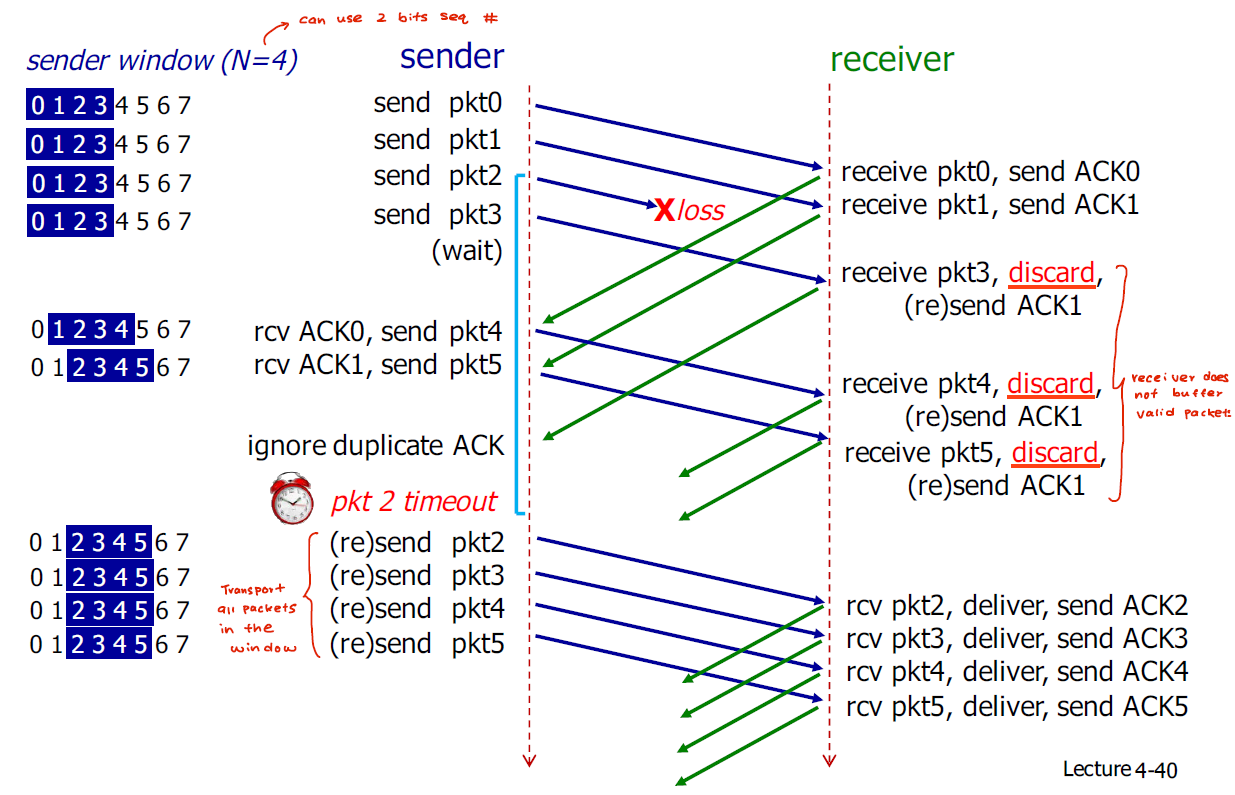
\includegraphics[width=0.9\columnwidth]{go-back-n}
        \end{center}
        \subsubsection{Selective Repeat}
        \textbf{Pros}: Only retransmits unACKed pkts and buffer out-of-order pkts $\rightarrow$ more efficient use of resources, no need to retransmit so many pkt\\
        \textbf{Cons}: much more complex since need to maintain multiple timers for all the packets in the window
        \begin{center}
            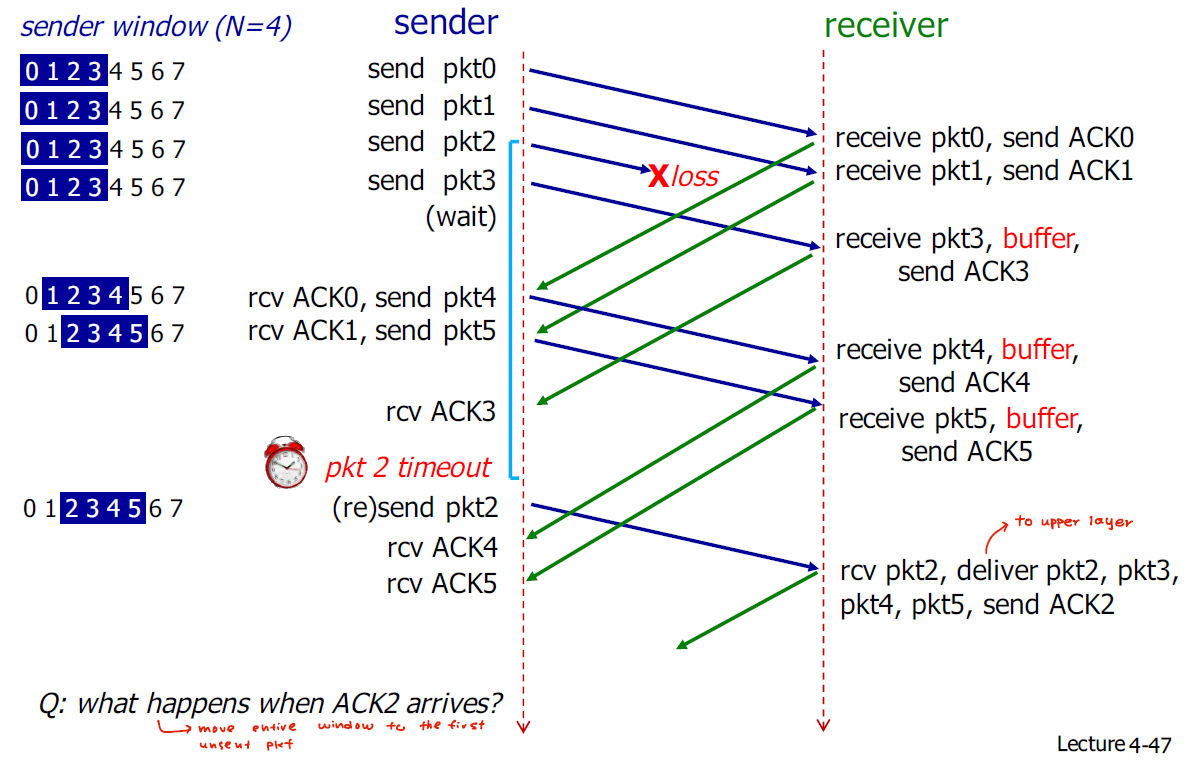
\includegraphics[width=0.85\columnwidth]{selective_repeat}
        \end{center}
        \section{Connection-oriented Transport: TCP}
        \begin{itemize}
            \item \textbf{Point-to-point}: 1 sender, 1 receiver
            \item \textbf{Connection-oriented}: handshake before data exchange
            \item \textbf{Full duplex data}: bi-directional data flow in same connection
            \item \textbf{Reliable, in-order \textcolor{red}{byte} stream}: no ``message boundaries'' (i.e. format of data sent does not matter $\rightarrow$ whether its a .jpg or .txt file, both is seen as stream of bytes)
            \item \textbf{Pipelined}: \textbf{dynamic} window size set by congestion/flow control
        \end{itemize}
        \subsection{TCP: buffers and Segments}
        \begin{itemize}
            \item two buffers: send and receive, created after handshaking at both sides. Buffers are regarded as a \textcolor{red}{stream of bytes}
            \item \textbf{Max Segment Size (MSS)}: typically 1460 bytes, max app-layer data one TCP segment can carry.
            \item Limited by maximum transmission unit (MTU), largest link-layer frame e.g. 1500 bytes for Ethernet
        \end{itemize}
        * Why 1460 Bytes specifically? Max = 1500 bytes, 20 bytes for IP header, 20 bytes for TCP header
        \subsection{Connection-oriented de-multiplexing}
        A TCP connection/socket is identified by 4-tuple \texttt{(srcIPAddr, srcPort, destIPAddr, destPort)}. If there are multiple connections to same destination port and address number, with different source IP and/or source port\#, server demultiplex connections to different sockets.\\\\
        * Note that server is usually threaded so that it can handle multiple connections
        \subsection{TCP Segment}
        \begin{center}
            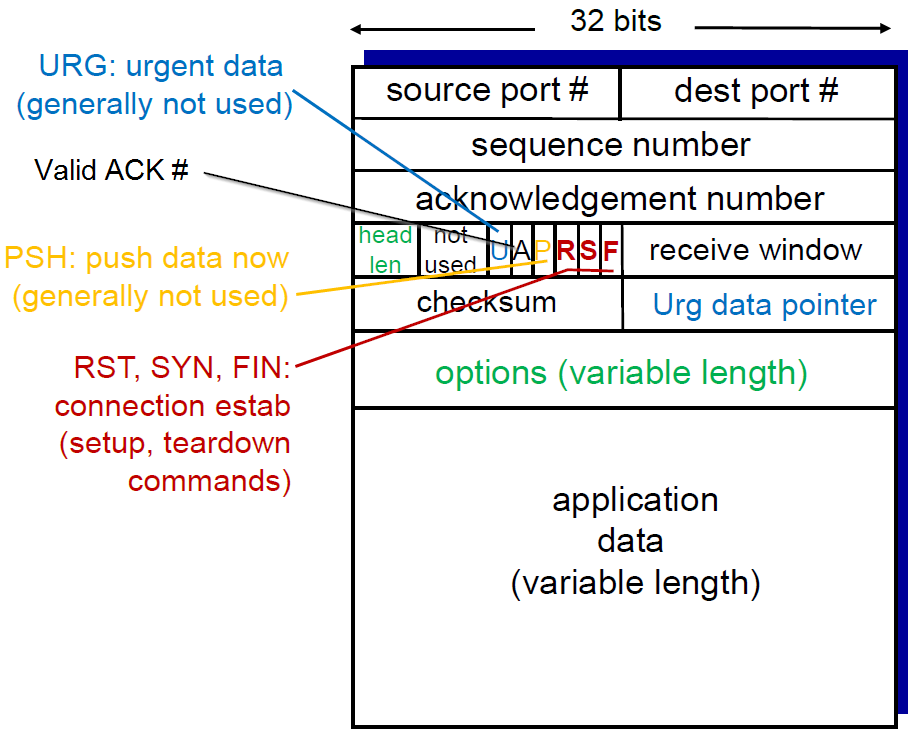
\includegraphics[width=0.7\columnwidth]{tcp_segment}
        \end{center}
        \begin{itemize}
            \item \textbf{Sequence Number}: \textcolor{red}{byte number} of the first byte of data in a segment (if it exceeds $2^{32} - 1$ then it will wrap around back to 0).
            \begin{itemize}
                \item Seq\# of sender and receiver is different and is \textcolor{red}{randomly picked} at the start of the connection (to prevent confusion during packet reorder)
                \item if we have a file of 500,000 bytes, MSS = 1000 bytes, then SEQ\# will be 1000, 2000, ...
            \end{itemize}
            \item \textbf{ACK number}: sequence number of the next byte of data expected by the receiver. Uses cumulative ACK (similar to go-back-N). \textcolor{red}{ACK\# = client\_seq\# + len(data)}
            \begin{itemize}
                \item Allows for \textbf{piggy-backing}: can send data along with ACK. ACK will be processed as long as ACK bit is 1.
                \item \textbf{Delayed ACK}: Receiver can wait up to 500ms for the next segment before sending an ACK (saves 1 cycle of ACK)
            \end{itemize}
            \item \texttt{\textbf{ACK}} bit: indicates whether segment includes an ACK and whether acknowledgement \# is valid. If ACK bit is 0, indicates that segment is a pure data segment
            \item \texttt{\textbf{SYN}} bit: used to signal a request for connection setup
            \item \texttt{\textbf{FIN}} bit: used to signal connection tear down
            \item \textbf{Receive Window}: \# of bytes rcvr willing to accept
        \end{itemize}
        * Note that TCP specifications doesn't say how to handle out-of-order segments, but it is usually buffered in practice (similar to selective repeat)
        \subsubsection{Example of transmission of TCP segment}
        \begin{center}
            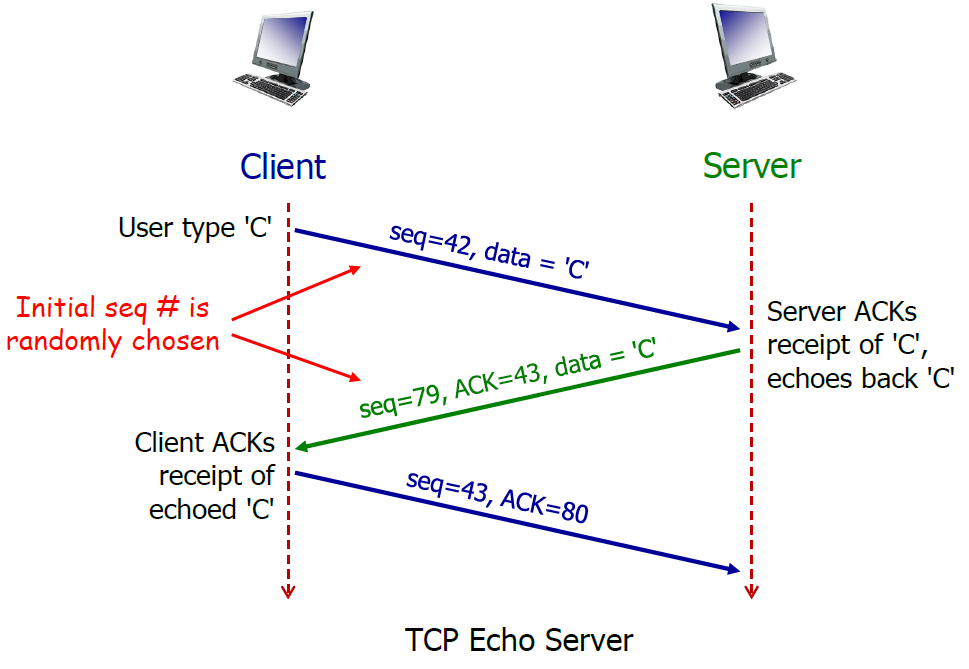
\includegraphics[width=0.7\columnwidth]{tcp_segment_eg}
        \end{center}
        \subsection{TCP Flow Control}
        Flow control allows rcvr to control sender, making sender dynamically change the window size so that rcvr's buffer won't overflow.\\
        Steps involved:
        \begin{enumerate}
            \item receiver ``advertises'' free buffer space (receive window in header (\texttt{rwnd}), typically defaults to 4096 bytes)
            \item sender limits amount of unacked data to rcvr's \texttt{rwnd} value
            \item this mechanism will hence guarantee rcvr buffer will not over flow and prevents data loss due to buffer overflow
        \end{enumerate}
        \subsection{TCP 3-way handshake}
        \subsubsection{TCP Set-up}
        \begin{center}
            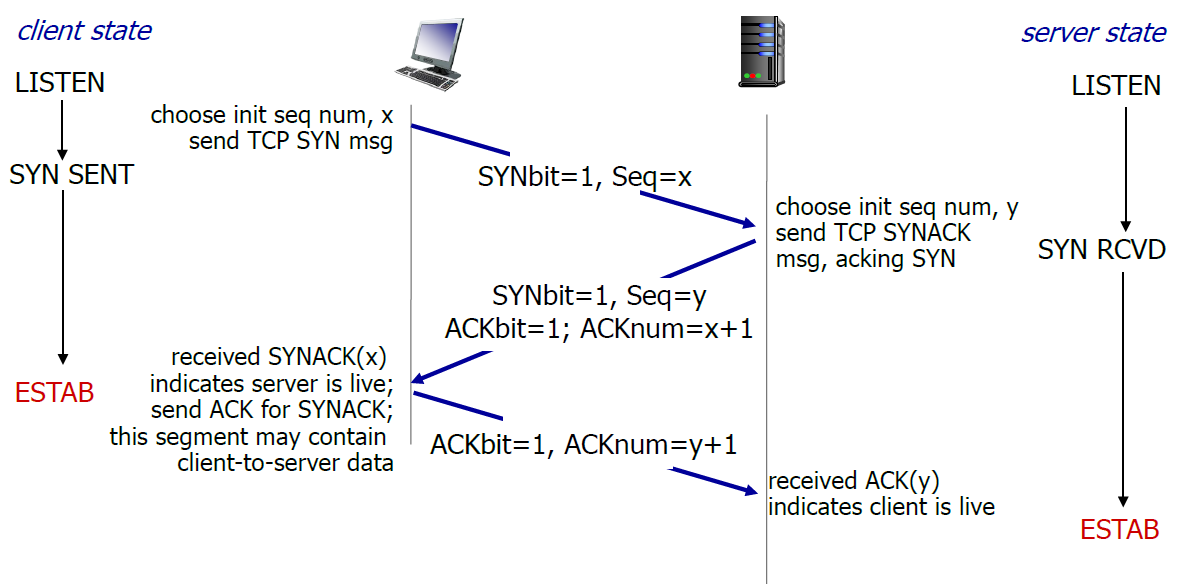
\includegraphics[width=0.75\columnwidth]{tcp_setup}
        \end{center}
        \subsubsection{TCP Tear-down}
        \begin{center}
            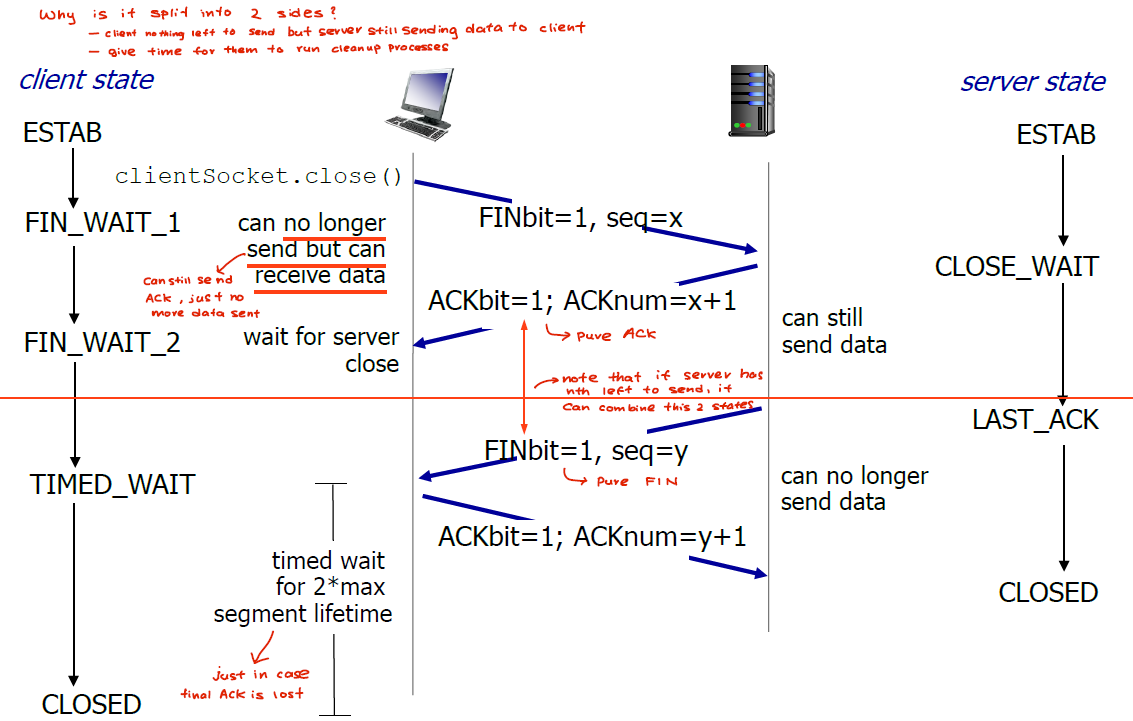
\includegraphics[width=0.9\columnwidth]{tcp_teardown}
        \end{center}
        \subsection{TCP RDT}
        \begin{itemize}
            \item TCP creates rdt service on top of IP's udt service: pipelined segments, cumulative acks, single retransmission timer, checksums
            \item Retransmissions triggered by: timeouts, duplicate ACKs
        \end{itemize}
        \begin{center}
            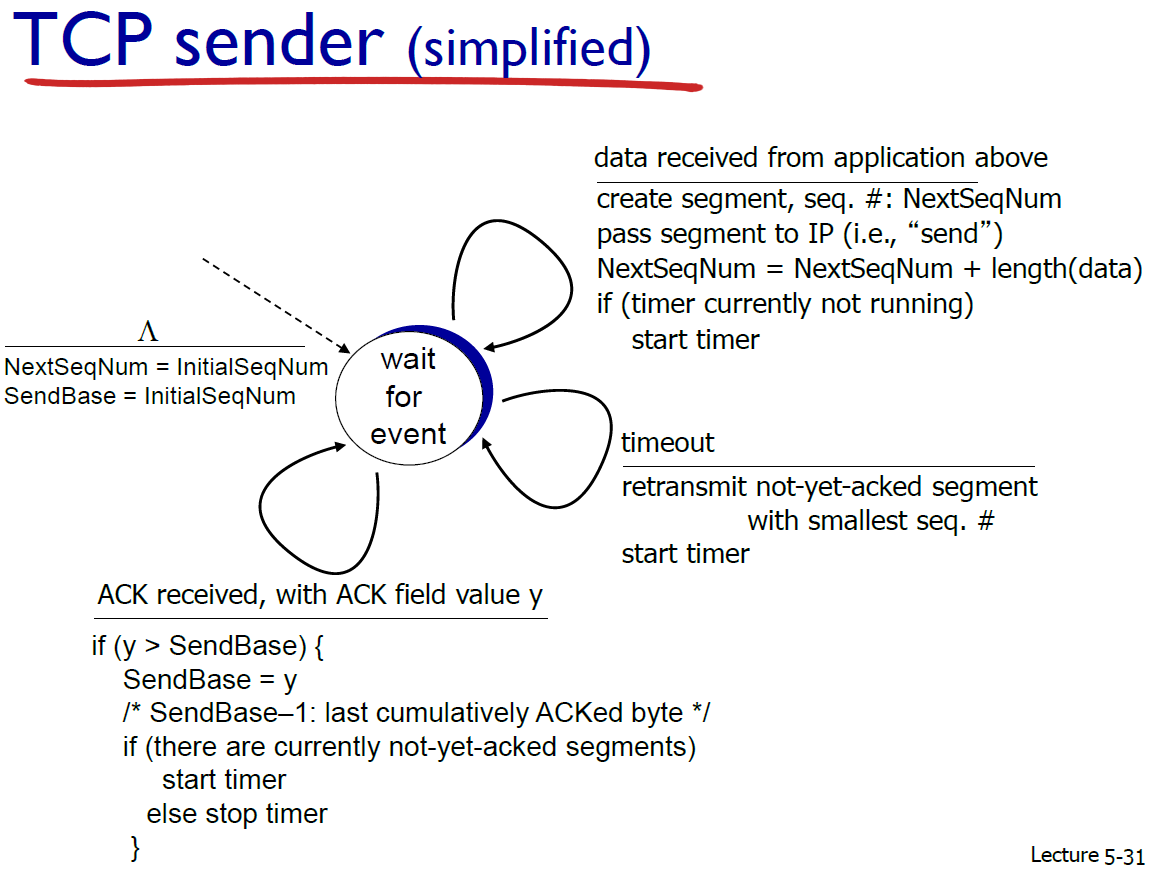
\includegraphics[width=0.8\columnwidth]{tcp_fsm}
        \end{center}
        \subsubsection{TCP ACK Generation}
        \begin{center}
            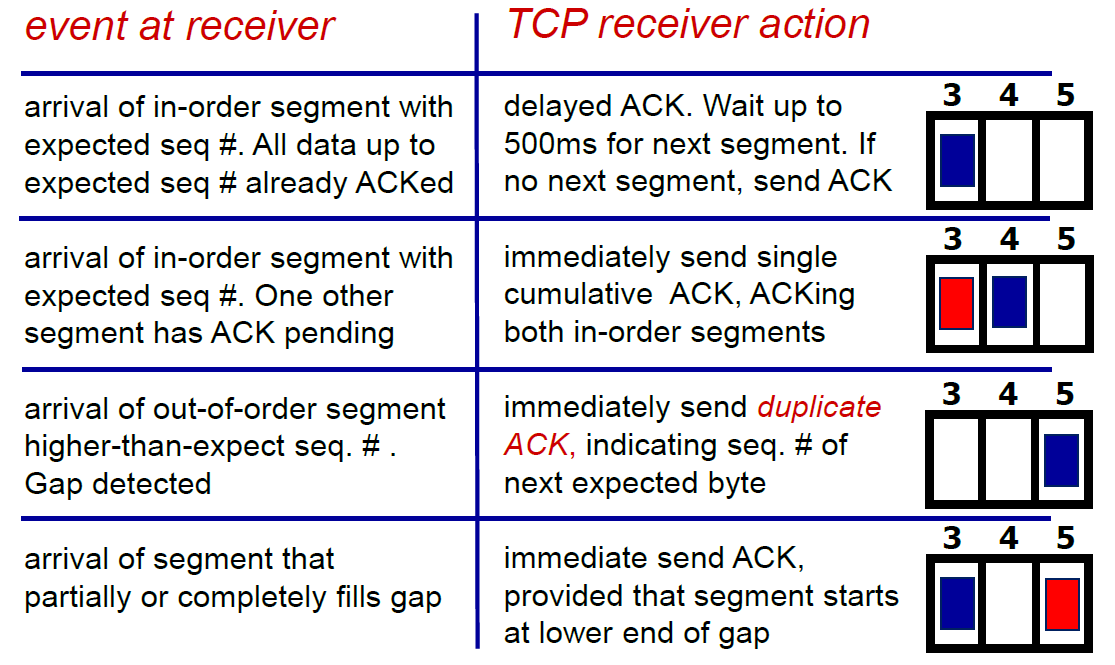
\includegraphics[width=0.8\columnwidth]{tcp_ack_gen}
        \end{center}
        \subsection{TCP Timeout}
        Considerations:
        \begin{itemize}
            \item Must be longer than RTT but RTT varies
            \item too short: premature timeout, unnecessary retransmissions
            \item too long: slow reaction to segment loss
        \end{itemize}
        Important equations:\\
        $EstimatedRTT = (1-\alpha)\times{EstimatedRTT} + \alpha\times{SampleRTT}$\\
        $DevRTT = (1-\beta)*DevRTT+\beta*|SampleRTT-EstimatedRTT|$\\
        $TimeoutInterval = EstimatedRTT + 4*DevRTT$
        \begin{itemize}
            \item exponential weighted moving average
            \item influence of past sample decreases exponentially fast
            \item typical value of $\alpha$ = 1/8
            \item typically $\beta$ = 1/4
        \end{itemize}
        \subsection{TCP fast retransmit}
        \begin{center}
            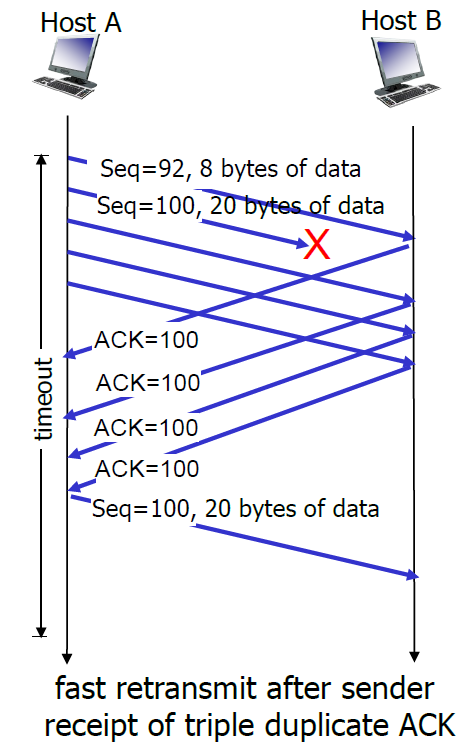
\includegraphics[width=0.25\columnwidth]{tcp_fast_retransmit}
        \end{center}
        \section{Miscellaneous}
        \textbf{Cookies Illustration}
        \begin{center}
            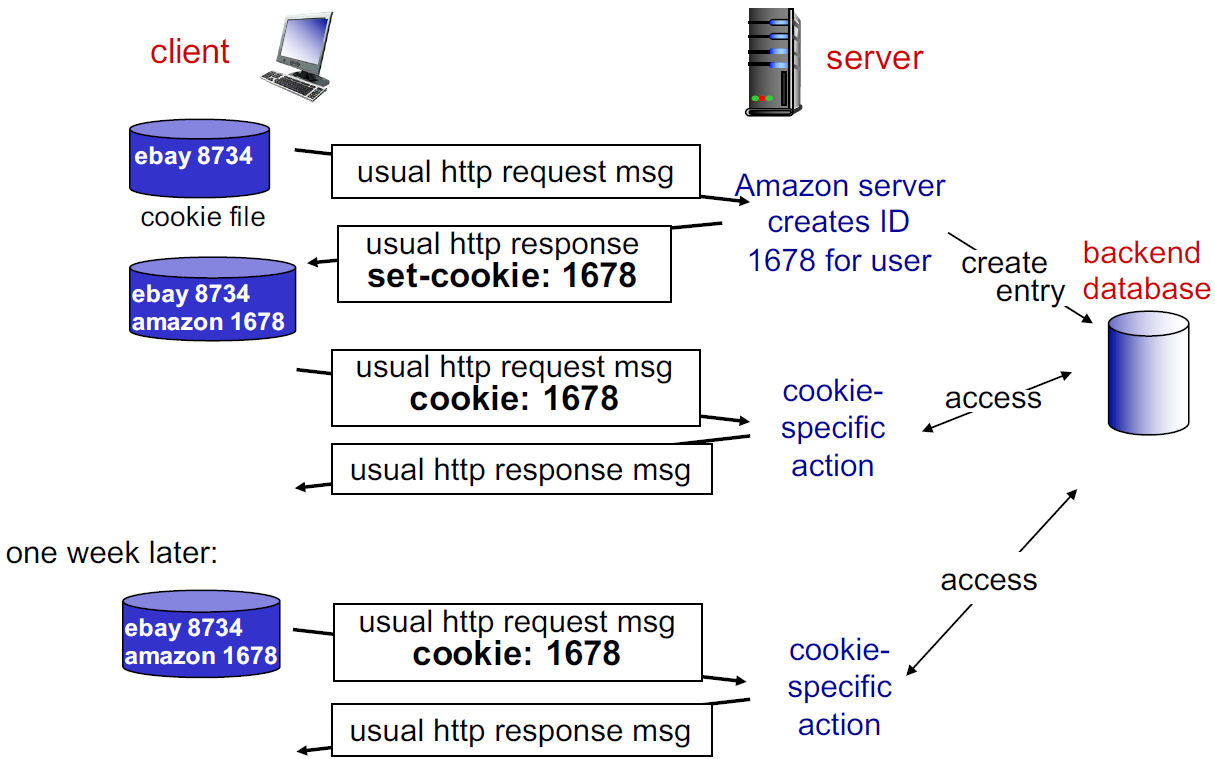
\includegraphics[scale=0.23]{cookies}
        \end{center}
        \textbf{RDT Summary}
        \begin{center}
            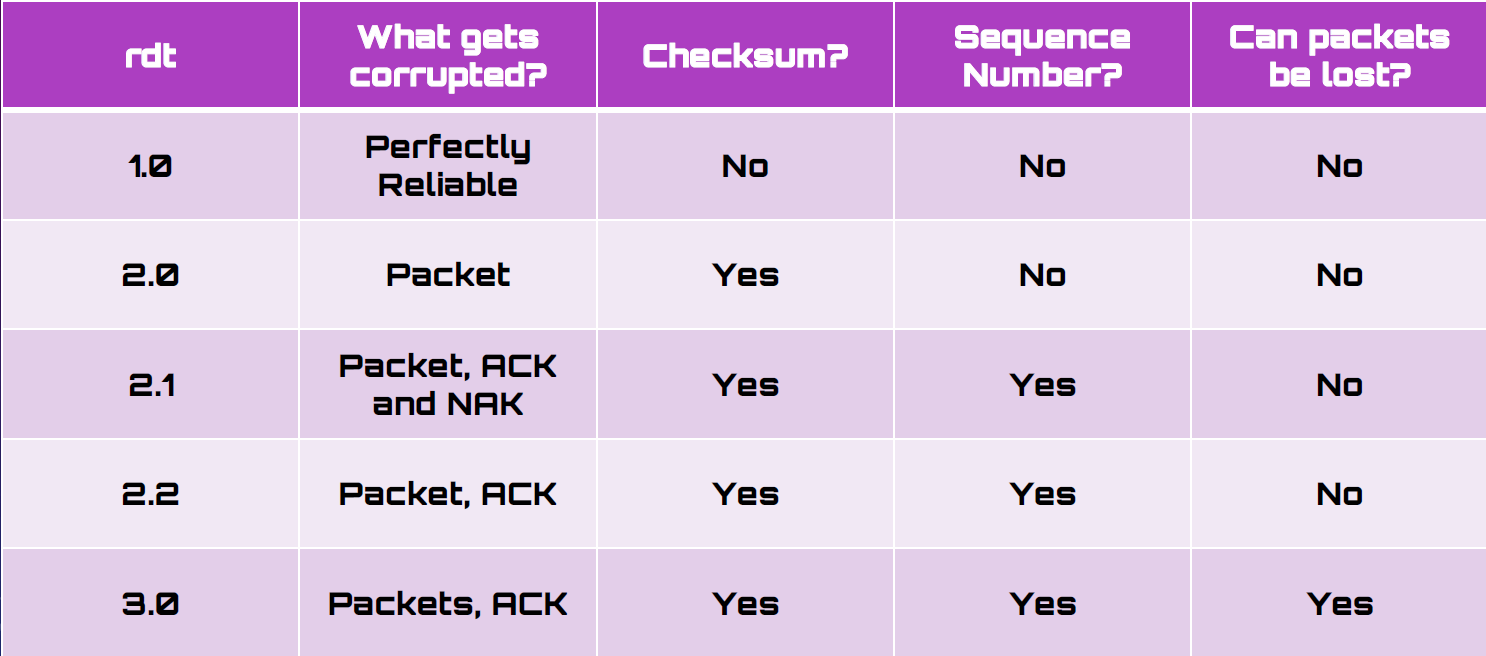
\includegraphics[width=0.9\columnwidth]{rdt_summary}
        \end{center}
        \textbf{Packet Reordering Issues using RDT3.0}\\
        Solution is to increase \texttt{seq\#} to hold more than 2 bits; use TTL to limit the lifespan of packets so that by the time \texttt{seq\#} is reused, TTL of old packet expires; Use random \texttt{init} seq\#
        \begin{center}
            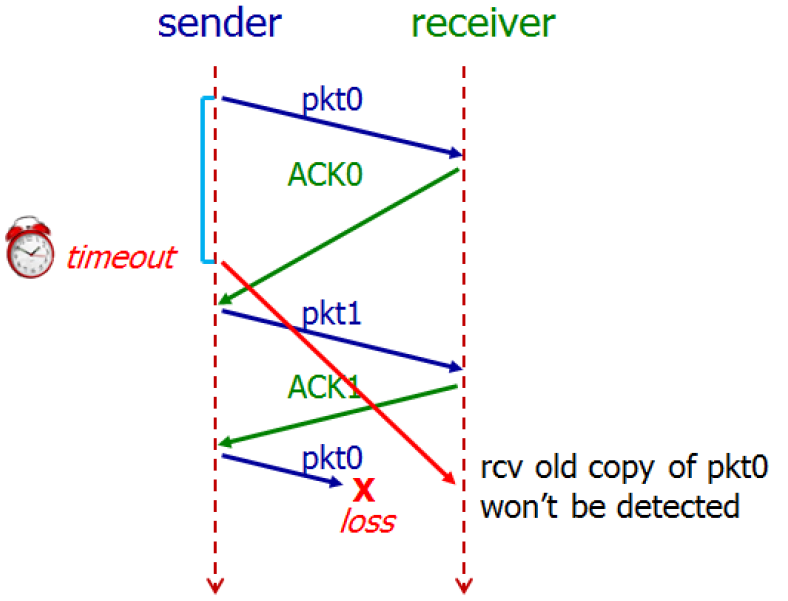
\includegraphics[width=0.5\columnwidth]{packet_reorder}
        \end{center}
        \textbf{TCP Retransmission Scenarios}
        \begin{center}
            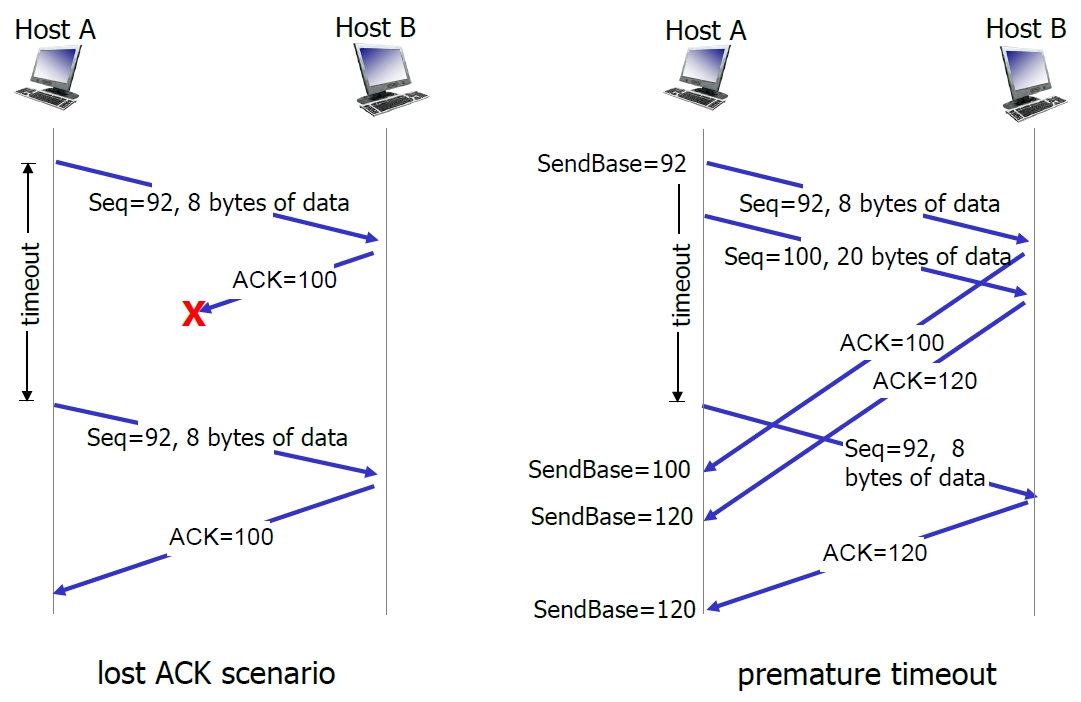
\includegraphics[width=0.7\columnwidth]{tcp_retransmission_1}
        \end{center}
        \begin{center}
            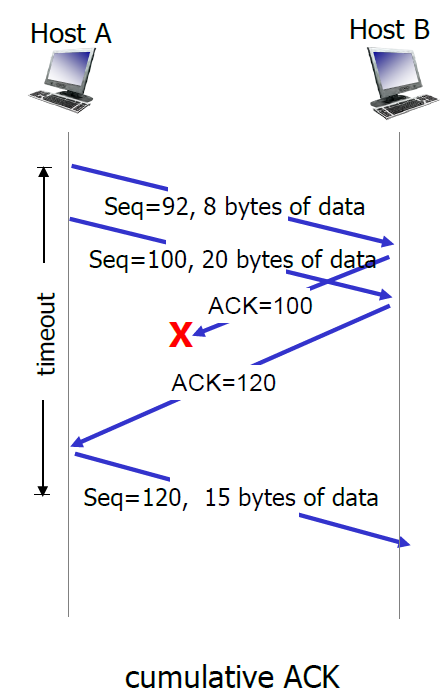
\includegraphics[width=0.3\columnwidth]{tcp_retransmission_2}
        \end{center}
        \textbf{Pipe-lining Summary}
        \begin{center}
            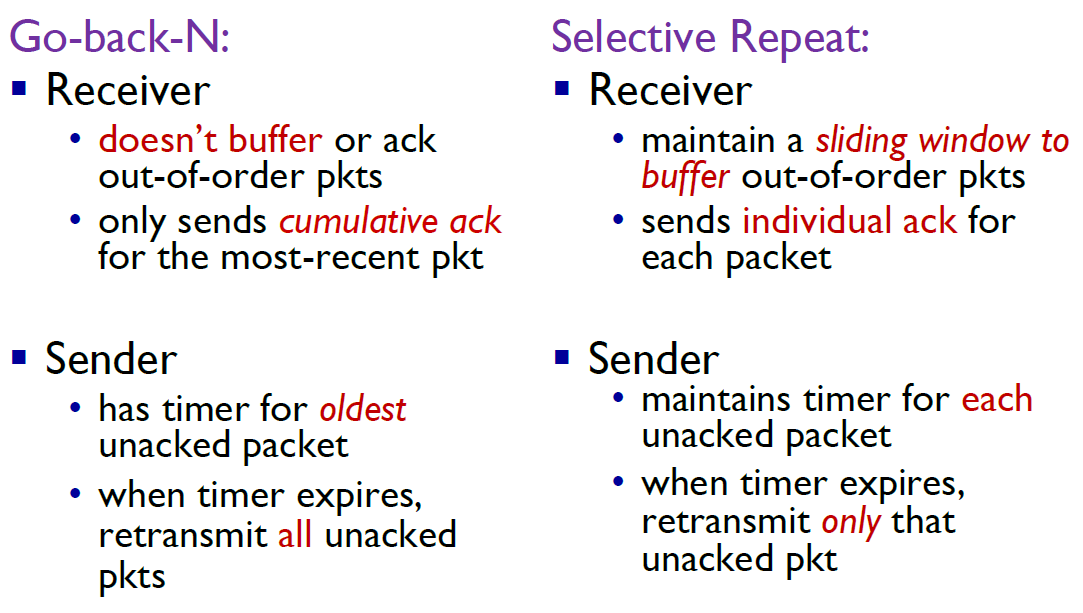
\includegraphics[width=0.9\columnwidth]{gbn_sr_summary}
        \end{center}
        \textbf{UDP Socket Illustration}
        \begin{center}
            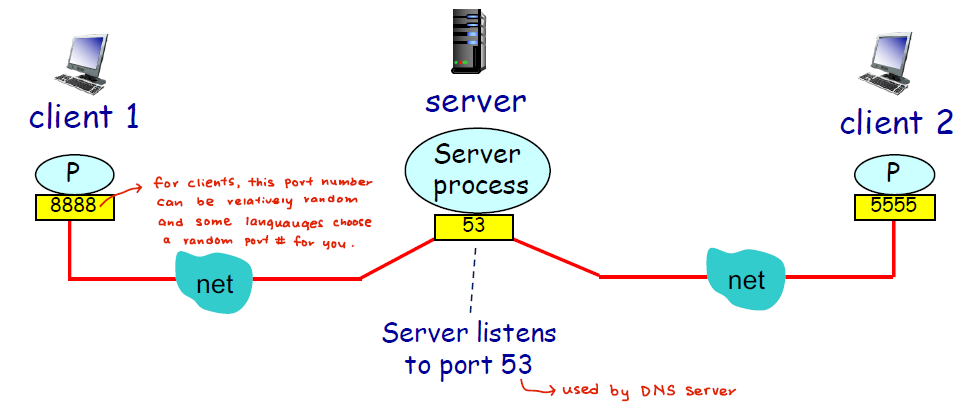
\includegraphics[width=0.9\columnwidth]{udp_socket}
        \end{center}
        \textbf{TCP Socket Illustration}
        \begin{center}
            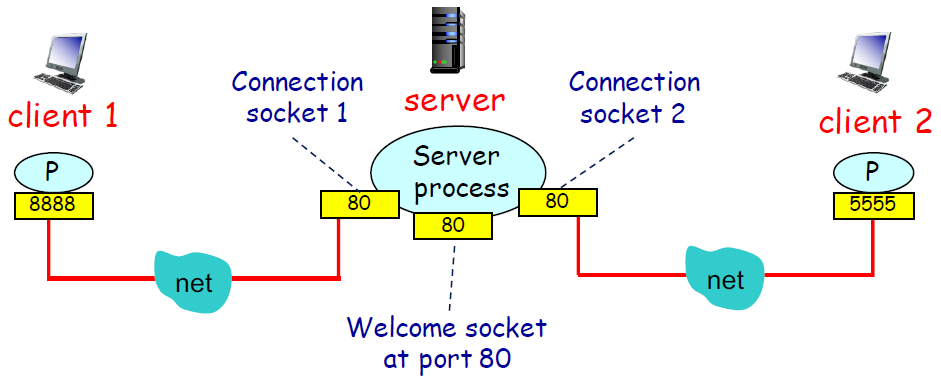
\includegraphics[width=0.9\columnwidth]{tcp_socket}
        \end{center}
        \textbf{Throughput vs Latency}
        \begin{itemize}
            \item \textbf{Latency}: how much time needed for information to be sent across to end user. (e.g. if someone on zoom speaks, how long does it take for other people to hear it?)
            \item Low latency important for live streaming service (e.g. Zoom, Twitch)
            \item \textbf{Throughput}: amount of data received in a given time period (e.g. When streaming Netflix, you need a throughput of say 5Mbps)
            \item Throughput does not account for delay (e.g. when streaming Netflix, you can allow for it to buffer for a few minutes, don't have to be live)
        \end{itemize}
    \end{multicols*}
\end{document}